% Please do not change the document class
\documentclass{scrartcl}

% Please do not change these packages
\usepackage[hidelinks]{hyperref}
\usepackage[none]{hyphenat}
\usepackage{setspace}
\usepackage{graphicx}
\graphicspath{ {Figures/} }
\doublespace

% You may add additional packages here
\usepackage{amsmath}

% Please include a clear, concise, and descriptive title
\title{Convexity-Based Collision Detection Algorithms for a 2D Platform Games}

% Please do not change the subtitle
\subtitle{COMP110 - Computer Architecture Essay}

% Please put your student number in the author field
\author{1507866}

\begin{document}
	
\maketitle
	
\abstract{This essay will analyse three convexity based collision detection algorithms focusing on both their accuracy and run times. Then a recommendation will be made based on which algorithm balances the two in the best way for use in a 2D platform game.}
%Add figures
%Add Minkowski textbook
%Change intended
	
\section{Introduction}
	
The purpose of collision detection is to check if objects are currently or going to intersect. In the application of video games this is vital for ensuring that objects interact correctly so the game can be played as it was intended.  This essay will analyse three convexity-based collision detection algorithms for use in a 2D platform game.  The first algorithm is the Gilbert- Johnson– Keerth algorithm first proposed in 1988. Guo proposed the second algorithm in 2010 and the third is by Sulaiman et al in 2013. One of these will be recommended based on its balance between accuracy and run time.

	
\section{The three algorithms}
\subsection{Algorithm One: ‘Gilbert-Johnson-Keerth’ (GJK) algorithm}
Gilbert et al proposed their collision detection algorithm, the ‘Gilbert- Johnson– Keerth’ (GJK) algorithm in 1988 \cite{GJK}. The algorithm is designed to work efficiently for 3D collision detection however it also works for 2D. Therefore it could be implemented in a 2D platform game. The intention of this algorithm is to determine whether objects intersect. This is done by calculating the Eucildean distance between a set of convex objects. According to Gilbert et al the distance between two convex objects is the same as the distance between those object’s Minkowski difference and the origin. If that difference is zero then the objects are intersecting each other or have collided.
\newline 
The original paper gives run times for the algorithm on a selection of 3D shapes. The minimum time being 0.13 seconds and the maximum being 19.81. However these are being run in 3D so it is likely it would take less time on 2D convex objects. Furthermore this paper was published in 1988 so the results are restricted by the technology of that time. The results from the paper are from tests run on a Harris 800 which was a computer available from 1979 \cite{harris800}. If the tests were repeated on modern hardware it would most likely run considerably faster.

The GJK algorithm is a very accurate algorithm due to its use of convex hulls. However the cost of this accuracy is speed. In the application of a 2D platform game speed is vital, a few seconds lag for each collision would make the game unplayable. While accuracy is important it should be balanced with speed for games.

An issue with the GJK algorithm could also be its age, there are a number of papers that recommend and detail improvements that could be made to GJK to make it faster or more efficient. Gilbert later detailed improvements for GJK in another in a paper in 1990. \cite{Gilbert2}.  Lindemann says that there is a sub-algorithm in GJK that is ''somewhat outdated'' \cite{lindemanngjk} but that particular algorithm is often replaced or adapted when used to fit the given situation.
	
\subsection{Algorithm Two: Guo's algorithm for 2D grapple games}
The second algorithm is designed for collision detection in 2D grapple games. This paper was published in 2010 making it more recent than the GJK algorithm however it is limited to 2D. In contrast GJK can work in m-dimensions, the paper detailed it’s use for three dimensions but it is also viable in 2D.  
	
Guo \cite{Guo} proposes a method which bounds the game objects in axis aligned rectangles and circles. A collision has occurred if there is an overlap region between the shape's detection area.
	
In this algorithm the detection area is the area inside of the bounding objects such as the rectangles and circles.  Data such as the coordinate systems are stored in data files beforehand and then loaded into the detection module while it is running.
	
This algorithm works by setting coordinate values for the rectangle and its four vertices.  The algorithm then calculates the distance between the shape centre and another point. This distance is used to see if any of the shapes vertices are enclosed in another object, if any vertices are then a collision is taking place. This algorithms result is a Boolean that states that either a collision is happening or not.
	
The evidence presented shows that this is a fast algorithm compared to GJK. The fastest results were for the collisions of two circles. The minimum and maximum time for that collision was 6.20531 milliseconds. The longest this algorithm took  was 160.105 milliseconds for the collision of two rectangles.  In contrast the GJK algorithm took a maximum of 19.91 seconds.  The results suggest it is faster than the GJK algorithm but the results for GJK were from 3D testing.
	
An issue with Guo's algorithm could be that it is specific to 2D grapple games. It may be unsuitable for use in other games or require some adaptation. In contrast the GJK algorithm is more open to general use as it can be used in 2D or 3D and is not just limited to use in games.
	
Sulaiman et al \cite{Sulaiman} suggested that the use of bounding boxes in collision detection can be inaccurate. This is because the bounding boxes may intersect and report that a collision is happening. However in actual fact the objects themselves are not colliding making the results inaccurate.
	
	
\subsection{Algorithm Three: Collision Detection using a dynamic origin point }
The third technique has been proposed by Sulaiman et al\cite{Sulaiman}. The algorithm is for distance computation in the narrow phase of two phase collision detection. The basis of this algorithm was to find a solution that was more accurate than bonding boxes. Their method involves using a dynamic origin point, or DyOp. Figure 1 demonstrates the first stages of DyOp.
\begin{figure}[h]
	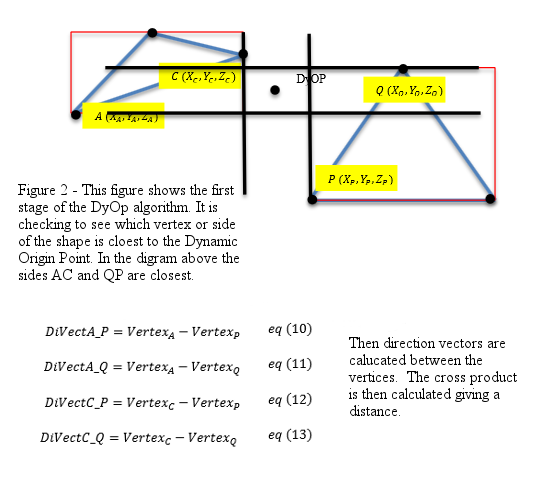
\includegraphics[width=1.0\linewidth]{A3figure.png}
	\caption{Figure 1. DyOp being used on two triangles \cite{Sulaiman}}
\end{figure}
\newline
\newline	
Sulaiman et al do not give run times for their algorithm. They instead compared it to two existing algorithms. One of which was the GJK  algorithm. They found that their algorithm gave a speed increase  between 78.1\% to 110.9\%. The DyOp algorithm does not provide data on how fast the algorithm is in milliseconds making it hard to compare to the second algorithm proposed by Guo. However Guo’s algorithm used bonding boxes. Sulaiman et al were aiming to implement an algorithm more accurate than bounding boxes.
%expand
	
Sulaiman et al's method is more accurate than using bonding boxes and is significantly faster than the GJK algorithm therefore based on the evidence given Sulaiman et al's DyOp algorithm is most suited for use in the 2D platform game. The lack of time data means it is not possible to tell whether it is faster than Guo or not. However Guo uses bonding boxes which while being fast leads to inaccuracy due to the way objects are bound.  
	
		
	
\section{Conclusion}
In conclusion the DyOp algorithm proposed by Sulaiman et al appears to be the best choice for the 2D platform game. DyOp performed significantly faster in tests than GJK and is more accurate than Guo's bounding box based algorithm. This balance between accuracy and speed makes it the ideal choice for use in a 2D platform game.  
	
	
\bibliographystyle{ieeetr}
\bibliography{comp110_architecture}
	
\end{document}
